\section{Introducción}
La \textbf{trigonometría} se dedica al estudio de las medidas de los triángulos 
y su relación entre ellas.
Dichas medidas son básicamente:
\begin{itemize}
  \item Lados y
  \item Ángulos
\end{itemize}

Por otra parte, un \textbf{triángulo} se define como una figura plana de tres 
lados. Además de los lados y los ángulos, un triángulo presenta una tercera 
propiedad llamada \textit{vértice}.
Los \textbf{vértices} son simplemente puntos que se unen mediante segmentos de recta para
poder formar un triángulo.

\begin{marginfigure}[-3.5cm]
	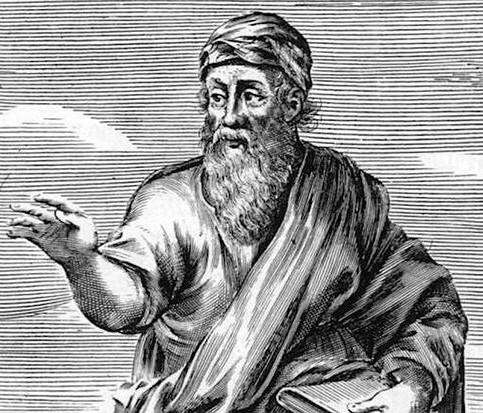
\includegraphics{pythagoras_cropped}
	\caption[pythagoras]{Pitágoras. Filósofo y matemático griego distinguido por 
    sus aportaciones a la artimética, geometría y trigonometría.
    % \\ 
	  % \url{https://www.pinterest.com/pin/133841420159654763/}
  }
	\labfig{pythagoras}
\end{marginfigure}

\subsection{Notación para nombrar triángulos}

Un triángulo puede ser nombrado con ayuda de sus vértices, de esta manera el 
triángulo de la figura \reffig{triangulo} se denota como el triángulo ABC que se 
representa como:
$$\widetriangle{ABC}$$

\begin{figure}[hb]
	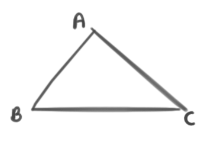
\includegraphics[width=0.40\textwidth]{triangulo}
	\caption[Triangulo]{Triángulo ABC. }
	\labfig{triangulo}
\end{figure}

\paragraph{Aspectos interesantes de la trigonometría}
\begin{itemize}
  \item Es una de las ramas de la matemática más antigua, su estudio se remonta 
  a la época griega en donde su exponente principal fue \textit{Pitágoras}, pese 
  a que oficialmente se reconozca a \textit{Hiparco de Nicea} como el padre de 
  la trigonometría.

  \item Los triángulos son los polígonos más simples
  \begin{itemize}
    \item Por ende carecen de diagonales
  \end{itemize}

  \item Para el estudio de otros polígonos se suele utilizar el método de 
  \textit{triángulación}, que se refiere básicamente a dividir dicha figura en 
  un conjunto ordenado de triángulos.
  %TODO:- Agregar la etimologia
\end{itemize}

% pseudo referencias 
% https://concepto.de/triangulo/